\documentclass[11pt, letterpaper]{article}

% ---------- packages ----------
\usepackage[margin=0.7in]{geometry}
\usepackage{tcolorbox}
\usepackage{enumitem}
\usepackage{hyperref}
\usepackage{xcolor}
\usepackage{titlesec}
\usepackage{fancyhdr}
\usepackage{graphicx}
\usepackage{tabularx}
\usepackage{booktabs}

% ---------- colors ----------
\definecolor{boxborder}{RGB}{60, 90, 150}
\definecolor{boxbg}{RGB}{245, 248, 255}
\definecolor{headcolor}{HTML}{00636f}
\definecolor{placeholder}{RGB}{140, 140, 140}

% ---------- tcolorbox style ----------
\tcbset{
  sectionbox/.style={
    colframe=boxborder,
    colback=boxbg,
    boxrule=0.6pt,
    arc=2pt,
    left=6pt, right=6pt, top=4pt, bottom=4pt,
    fontupper=\small,
  }
}

% ---------- placeholder command ----------
\newcommand{\placeholder}[1]{\textcolor{placeholder}{\textit{#1}}}

% ---------- section formatting ----------
\titleformat{\section}
  {\normalsize\bfseries\color{headcolor}}{\thesection.}{0.4em}{}
\titlespacing*{\section}{0pt}{6pt}{2pt}

% ---------- header / footer ----------
\pagestyle{fancy}
\fancyhf{}
\renewcommand{\headrulewidth}{0.4pt}
\lhead{\small\color{headcolor} CS 4100 -- Project Executive Summary}
%\rhead{\small\color{headcolor} Semester, Year}
\cfoot{\small\thepage}

% ---------- suppress paragraph indent ----------
\setlength{\parindent}{0pt}
\setlength{\parskip}{3pt}

\begin{document}

% ===== TITLE BLOCK =====
\begin{center}
  {\Large\bfseries\color{headcolor} Project Title Here}\\[4pt]
  {\normalsize Member 1, Member 2, Member 3, Member 4}\\[2pt]
\end{center}

\vspace{4pt}

% ===== 1. MOTIVATION & PROBLEM STATEMENT =====
\section{Motivation \& Problem Statement}
\begin{tcolorbox}[sectionbox, height=4.6cm, valign=top]
	Counter-Strike is a highly competitive first-person shooter game with a steep learning curve.
	Players must make fast decisions based on teammate location, timing, strategy usage, and incomplete knowledge of the enemy team.
	Existing tools such as the HLTV rating system aim to evaluate player performance.
	The scoring system considers aspects including average damage per round, deaths per round, KAST (Kill/Assist/Survive/Traded), and so on.
	However, this scoring system is not helpful in coaching the players in two ways.
	First, the rating is aggregated over an entire match, so the player is not able to identify which rounds or moments drove their score up or down.
	Also, the rating is based on the outcome of the player's actions, but not on the action itself.
	Such a system cannot tell players what caused their score to be low, or which action in a certain situation is not advised.

	Therefore, in this project, we aim to build a post-game AI coaching pipeline for Counter-Strike 2.
	After the player has completed a match, they can feed the demo file into the pipeline.
	Models in the pipeline are able to analyze the gameplay and compute the optimal purchasing recommendations and strategies to implement for each round.
	By comparing the output with the actual decisions made by the player, the pipeline can provide fine-grained round-level and event-level scores of how the player performed.
	From this fine-grained post-game analysis, players are able to identify their recurring weaknesses and build better intuition when facing the same scenarios.
\end{tcolorbox}

% ===== 2. APPROACH =====
\section{Approach}
\begin{tcolorbox}[sectionbox, height=7.0cm, valign=top]
% --> REMOVE THE \placeholder ENV BELOW, AND ADD YOUR OWN TEXT  <-- %
  \placeholder{%
    Summarize your technical approach at a high level. Describe the
    system architecture or methodology, key algorithms or models used,
    and the most important design decisions. If applicable, include a
    small figure or diagram (use \textbackslash includegraphics), and resize to stay within bounded box area.
    Mention the primary tools, frameworks, or libraries
    (e.g., PyTorch, Mesa, Gymnasium, PettingZoo).
    Clearly state any assumptions or scope limitations.
    Aim for roughly 10--15 sentences or equivalent with an optional figure.}
\end{tcolorbox}

% ===== 3. KEY RESULTS =====
\section{Key Results}
\begin{tcolorbox}[sectionbox, height=8cm, valign=top]
% --> REMOVE THE \placeholder ENV BELOW, AND ADD YOUR OWN TEXT  <-- %
  \placeholder{%
    Present the most important quantitative and/or qualitative results.
    Include 1--2 key metrics, comparisons, or summary statistics.
    Interpret the results: what worked well, what was surprising,
    and how do the outcomes compare with your initial expectations
    or baselines? Aim for roughly 8--12 sentences or equivalent. Small tables, figures, or charts may be embedded here, and/or in the first box on the next page (examples on next page).}
\end{tcolorbox}

\newpage

\begin{tcolorbox}[sectionbox, height=8cm, valign=top]
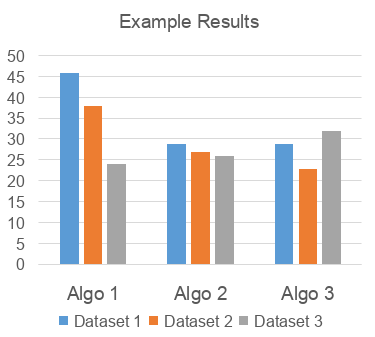
\includegraphics[width=0.42\linewidth]{Picture.png}\hfill
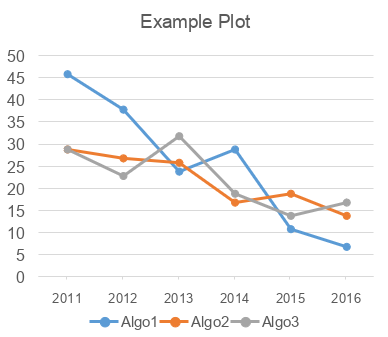
\includegraphics[width=0.42\linewidth]{Picture2.png}
  \\
  % --> REMOVE THE \placeholder ENV BELOW, AND ADD YOUR OWN TEXT  <-- %
  \placeholder{%
  Replace these figures with your own, or remove them and use this space for more text. Ensure all text in your figures are clear and readable at this scale, similar to these examples.
   }
\end{tcolorbox}
% ===== 4. CHALLENGES & LESSONS LEARNED =====
\section{Challenges \& Lessons Learned}
\begin{tcolorbox}[sectionbox, height=4.4cm, valign=top]
% --> REMOVE THE \placeholder ENV BELOW, AND ADD YOUR OWN TEXT  <-- %
  \placeholder{%
    Discuss the main technical and organizational challenges
    encountered during the project. For each challenge, briefly
    explain how the team addressed or mitigated it.
    Highlight lessons learned that would be valuable for future
    work or for other teams tackling similar problems.
    Aim for roughly 8--12 sentences.}
\end{tcolorbox}

% ===== 5. INDIVIDUAL CONTRIBUTIONS =====
\section{Individual Contributions}
\begin{tcolorbox}[sectionbox, height=4.3cm, valign=top]
% --> REMOVE THE \placeholder ENV BELOW BEFORE SUBMISSION  <-- %
  \placeholder{Replace the table below with your team's actual contributions.}

  \vspace{4pt}
  \centering
  \begin{tabularx}{0.95\textwidth}{l X c}
    \toprule
    \textbf{Member} & \textbf{Primary Contributions} & \textbf{Approx.\ \%} \\
    \midrule
    Member 1 & \placeholder{e.g., System design, agent logic}          & 20\% \\
    Member 2 & \placeholder{e.g., Data pipeline, evaluation scripts}   & 20\% \\
    Member 3 & \placeholder{e.g., Environment design and implementation} & 20\% \\
    Member 4 & \placeholder{e.g., Data pipeline, evaluation scripts}  & 20\% \\
    Member 5 & \placeholder{e.g., System design, agent logic}  & 20\% \\
    \bottomrule
  \end{tabularx}
\end{tcolorbox}

% ===== 6. REPOSITORY & REFERENCES =====
\section{Repository \& References}
\begin{tcolorbox}[sectionbox, height=4.5cm, valign=top]
  \textbf{GitHub Repository:}
  \placeholder{\href{https://github.com/your-org/your-repo}%
       {\texttt{https://github.com/your-org/your-repo}}}\\
    \placeholder{Ensure repo is public, or add instructor as a collaborator.}\vspace{1pt}

  \textbf{Project Tracker:} \placeholder{\href{https://github.com/your-org/your-repo}{\texttt{https://github.com/your-org/projects/your-project}}}

  \vspace{6pt}
  \textbf{Key References:}
  \begin{enumerate}[leftmargin=1.4em, itemsep=1pt, topsep=2pt, label={[\arabic*]}]
    \item \placeholder{Author(s), ``Title,'' Venue, Year. Brief annotation.}
    \item \placeholder{Author(s), ``Title,'' Venue, Year. Brief annotation.}
    \item \placeholder{Author(s), ``Title,'' Venue, Year. Brief annotation.}
  \end{enumerate}

  \vspace{4pt}
  \placeholder{Add or remove reference entries as needed (3--4 recommended).}
\end{tcolorbox}

\end{document}